
\section{least-squares fitting of cubic splines}
\label{sec:spline3method1}

Aqui é mostrado como encaixar a curva $f(x):\mathbb{R}\rightarrow \mathbb{R}$, 
 sobre um conjunto de $N$ pontos $(x_n,y_n)$,
$\forall n \in \mathbb{Z},~0\leq n < N$; mediante o uso de mínimos quadrados, tendo
cada ponto uma importância de $w_n$.
Onde a curva 
$y=f(x)$ esta composta de um grupo de $M$ splines cúbicos (polinômios de grau 3), 
como o exemplo da Figura \ref{fig:leastmeanspline3}.
\begin{figure}[!htb]
\centering
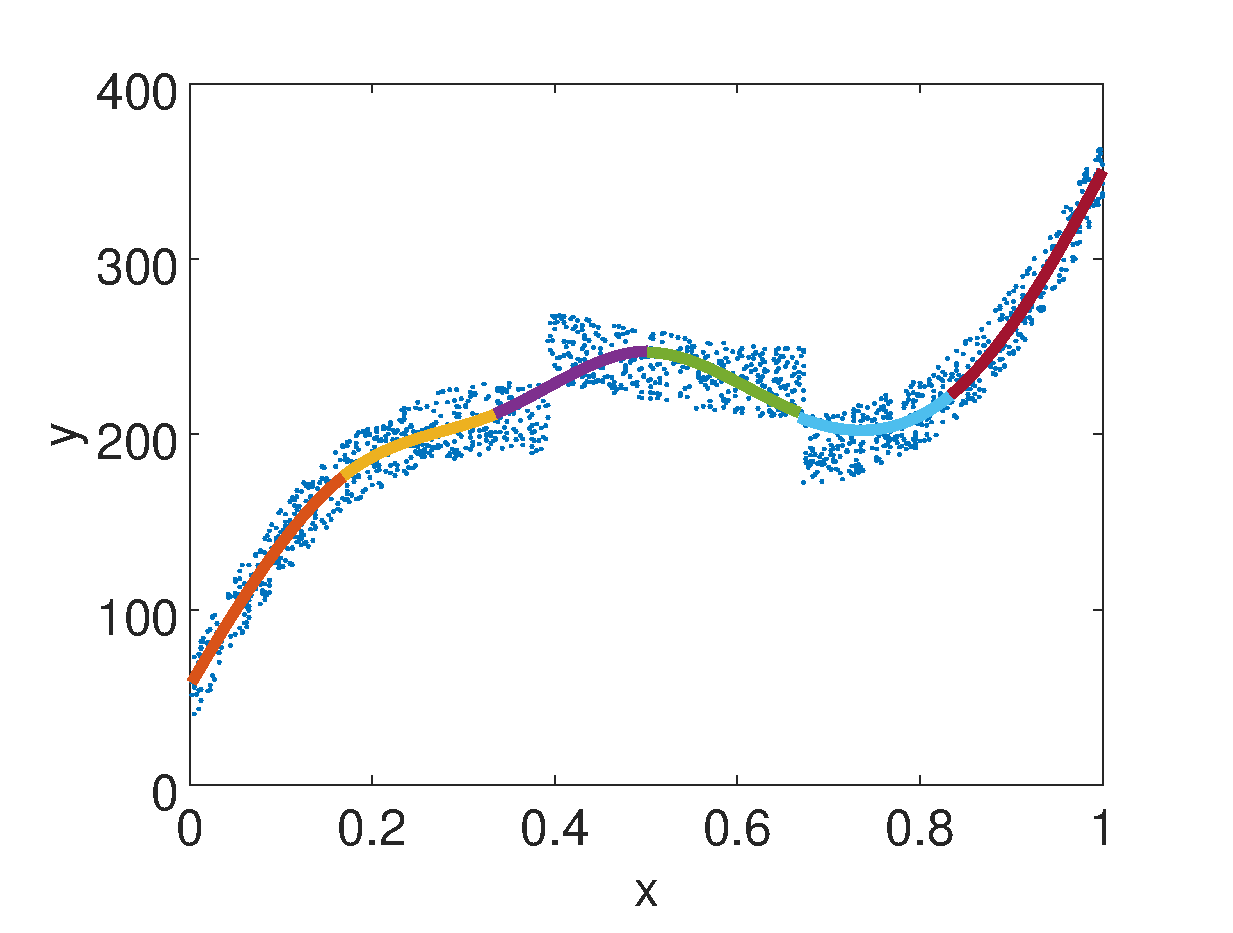
\includegraphics[width=0.6\textwidth]{section-cubic-splines/splines3demo.eps}
\caption{Encaixe de $M=6$ splines cúbicos num conjunto de $N=500$ pontos $\{x_n,y_n\}$.}
\label{fig:leastmeanspline3}
\end{figure}

Os splines tem seus limites de domínio, nas posições onde $x$ tem valores 
$d_{0}, d_{1}, d_{2}, ..., d_{M}$;
assim, podemos definir os vetores 
$\VECTOR{d}=\left(\begin{matrix}d_0 & d_1 & ...  & d_{M}\end{matrix}\right)^T$ $\in \mathbb{R}^{M+1}$ e
$\VECTOR{p}=\left(\begin{matrix}p_0 & p_1 & ...  & p_{4M-1}\end{matrix}\right)^T$ $\in \mathbb{R}^{4M}$,
de modo que podemos expressar $f(x)$ mediante
\begin{comment}
\begin{equation}
 G(x,a,b)= \left\{\begin{matrix}
1 & if &  a \leq x \leq b \\ 
0 & if & other~case
\end{matrix}\right.
\end{equation}
\end{comment}
o uso do polinômio cúbico
\begin{equation}
 S_k(x,\VECTOR{p})=P_{4k}~x^3+P_{1+4k}~x^2+P_{2+4k}~x+P_{3+4k},
\end{equation}
na função
\begin{comment}
\begin{equation}
 f(x,\VECTOR{p},\VECTOR{d})=\sum_{k=0}^{M-1} S_k(x,\VECTOR{p})G(x,d_{k},d_{k+1})  
\end{equation}
\end{comment}
\begin{equation}
f(x)\equiv f(x,\VECTOR{p},\VECTOR{d})= \left\{\begin{matrix}
S_0(x,\VECTOR{p}) & if & d_0 \leq x \leq d_1 \\ 
S_1(x,\VECTOR{p}) & if & d_1 \leq x \leq d_2 \\ 
S_2(x,\VECTOR{p}) & if & d_2 \leq x \leq d_3 \\ 
\vdots & \vdots & \vdots \\
S_{M-1}(x,\VECTOR{p}) & if & d_{M-1} \leq x \leq d_{M} \\  
\end{matrix}\right.
\end{equation}

%%%%%%%%%%%%%%%%%%%%%%%%%%%%%%%%%%%%%%%%%%%%%%%%%%%%%%%%%%%%%%%%%%%%%%%%%%%%%%%%
%%%%%%%%%%%%%%%%%%%%%%%%%%%%%%%%%%%%%%%%%%%%%%%%%%%%%%%%%%%%%%%%%%%%%%%%%%%%%%%%
\subsection{Calculando o vetor de parâmetros $\VECTOR{p}$}
Agrupando as $N$ amostras $\{x_n,y_n\}$ como mostrado na  Seção \ref{subsec:all}, 
podemos definir
\begin{equation}
\VECTOR{z}=
\left(\begin{matrix}
\VECTOR{y} \\
\mathbf{0} \\
\mathbf{0} \\
\mathbf{0} 
\end{matrix}\right),
\qquad 
\MATRIX{Q}=
\left(\begin{matrix}
\mathbf{A} \\
\MATRIX{B}_0 \\
\MATRIX{B}_1 \\
\MATRIX{B}_2 
\end{matrix}\right),
\qquad 
\MATRIX{R}=diag
\left(\begin{matrix}
\VECTOR{w} \\
\VECTOR{w}_a \\
\VECTOR{w}_b \\
\VECTOR{w}_c 
\end{matrix}\right);
\end{equation}
onde os vetores $\VECTOR{w}_a$, $\VECTOR{w}_b$ e $\VECTOR{w}_c$ são escolhido por nós,
e indicam o peso que desejamos dar ao cálculo do erro na continuidade de polinômios adjacentes,
na suas derivadas de ordem $0$, $1$ e $2$, respetivamente. 
Assim, para calcula o vetor $\VECTOR{p}$,  aplicamos $LMS$ (Least Mean Square)
definindo a  regra de minimização $e(\VECTOR{p}):\mathbb{R}^{4M}\rightarrow \mathbb{R}$,
\begin{equation}
 e(\VECTOR{p})=||\VECTOR{z} -\MATRIX{Q}  \VECTOR{p} ||_{\MATRIX{R}}^2+\alpha || \VECTOR{p}-\VECTOR{p}_{*} ||.
\end{equation}
Onde $\VECTOR{p}_{*}$ pode ser entendido como  $\VECTOR{p}$ numa iteração anterior; é dizer $\VECTOR{p}_{*}\equiv \VECTOR{p}_{k-1}$. Assim, aplicando
$LMS$ e a regularização de Tikhonov, o mínimo valor de $\VECTOR{p}=\VECTOR{\hat{p}}$ que minimiza $e(\VECTOR{p})$ 
se obtêm iterativamente usando a equação
\begin{equation}
\VECTOR{p}_{k}= \VECTOR{p}_{k-1}+ \left[ \MATRIX{Q}^T \MATRIX{R}\MATRIX{Q} +\alpha \mathbf{I} \right]^{-1} \MATRIX{Q}^T \MATRIX{R}  \left[ \VECTOR{z}-\MATRIX{Q}  \VECTOR{p}_{k-1} \right]
\end{equation}
desde um $\VECTOR{p}_{0}$ sabiamente escolhido,
ate que os vetores $\VECTOR{p}_{k}$ e $\VECTOR{p}_{k-1}$ sejam muito próximos,
onde se declara que $\VECTOR{\hat{p}}=\VECTOR{p}_{k}$. 



%%%%%%%%%%%%%%%%%%%%%%%%%%%%%%%%%%%%%%%%%%%%%%%%%%%%%%%%%%%%%%%%%%%%%%%%%%%%%%%%
%%%%%%%%%%%%%%%%%%%%%%%%%%%%%%%%%%%%%%%%%%%%%%%%%%%%%%%%%%%%%%%%%%%%%%%%%%%%%%%%
\subsection{Modelando a solução}
\label{subsec:all}
Para poder calcular o vetor $\VECTOR{p}=\left(\begin{matrix}p_0 & p_1 & p_2 & ...  & p_{4M-1}\end{matrix}\right)^T$, 
do problema spline descrito  na Seção \ref{sec:spline3method1}, a partir dos dados $(x_n,y_n,w_n)$; 
$\forall n \in \mathbb{Z},~0\leq n < N$,
é necessário escolher os valores $\VECTOR{d}=\left(\begin{matrix}d_0 & d_1 & ...  & d_{M}\end{matrix}\right)^T$;
ordenamos nossos dados nos seguintes vetores e sub-vetores coluna:
\begin{equation}
\VECTOR{x}=\left(\begin{matrix}\VECTOR{x}_0 \\ \VECTOR{x}_1 \\ \vdots  \\ \VECTOR{x}_{m}\\ \vdots  \\ \VECTOR{x}_{M-1}\end{matrix}\right),~~
\VECTOR{y}=\left(\begin{matrix}\VECTOR{y}_0 \\ \VECTOR{y}_1 \\ \vdots  \\ \VECTOR{y}_{m}\\ \vdots  \\ \VECTOR{y}_{M-1}\end{matrix}\right),~~
\VECTOR{w}=\left(\begin{matrix}\VECTOR{w}_0 \\ \VECTOR{w}_1 \\ \vdots  \\ \VECTOR{w}_{m}\\ \vdots  \\ \VECTOR{w}_{M-1}\end{matrix}\right),
\end{equation}
onde $\VECTOR{x}$, $\VECTOR{y}$ e  $\VECTOR{z}$ $\in \mathbb{R}^{N}$, e os sub-vetoes $\VECTOR{x}_m$, $\VECTOR{y}_m$ e $\VECTOR{w}_m$, incluem informação de $\{x_n,y_n,w_n\}$
que tem  domínio em $d_{m} \leq x_n \leq d_{m+1}$.


\subsubsection{Minimização do erro  $||\VECTOR{y} - \mathbf{A}\VECTOR{p}||^2_{\MATRIX{W}}$}
\label{subsubsec:partz}
Os dados $(x_n,y_n)$ são agrupados de forma que se procura minimizar $||\VECTOR{y} - \mathbf{A}\VECTOR{p}||^2_{\MATRIX{W}}$, 
onde a matriz diagonal $\MATRIX{W}=diag(\VECTOR{w})$,
\begin{equation}
\mathbf{A}_m =\left(\begin{matrix}
\VECTOR{x}_m^3 & \VECTOR{x}_m^2 & \VECTOR{x}_m & \mathbf{1}
\end{matrix}\right)
\end{equation}
\begin{equation}
\mathbf{A} =\left(\begin{matrix}
\mathbf{A}_0 & \mathbf{0}   & \mathbf{0}   & \dots & \mathbf{0} \\
\mathbf{0}   & \mathbf{A}_1 & \mathbf{0}   & \dots & \mathbf{0} \\
\mathbf{0}   & \mathbf{0}   & \mathbf{A}_2 & \dots & \mathbf{0} \\
\mathbf{0}   & \mathbf{0}   & \mathbf{0}   & \dots & \mathbf{A}_{M-1} \\
\end{matrix}\right) \in \mathbb{R}^{N \times 4M}
\end{equation}

\subsubsection{Minimização do erro $||\MATRIX{B}_0\VECTOR{p}||^2_{\MATRIX{W}_a}$ na derivada de ordem $0$ em splines adjacentes}
\label{subsubsec:part0}
Dados os polinômios $S_{k-1}(x,\VECTOR{p})$ e $S_{k}(x,\VECTOR{p})$ do $(k-1)$-ésimo e $k$-ésimo spline,
respetivamente. Podemos igualar ambos polinômios para garantir a continuidade dos splines em $x=d_{k}$, 
de modo que,
\begin{equation}
 S_{k-1}(d_{k},\VECTOR{p})=S_{k}(d_{k},\VECTOR{p}),
\end{equation}
Se agrupamos estas equações para os valores de  $0<k<M$, obtemos o sistema $\mathbf{0}=\MATRIX{B}_0 \VECTOR{p}$, 
onde $\MATRIX{B}_0 \in \mathbb{R}^{M-1 \times 4M}$ é definido como
\begin{equation}
\MATRIX{B}_0 =\left(\begin{matrix}
\VECTOR{e}_1 & -\VECTOR{e}_1   & \mathbf{0}    &  \mathbf{0}   & \dots & \mathbf{0} & \mathbf{0}\\
\mathbf{0}   &  \VECTOR{e}_2   & -\VECTOR{e}_2 &  \mathbf{0}   & \dots & \mathbf{0} & \mathbf{0}\\
\mathbf{0}   &  \mathbf{0}     &  \VECTOR{e}_3 & -\VECTOR{e}_3 & \dots & \mathbf{0} & \mathbf{0}\\
\vdots       &  \vdots         &  \vdots       &  \vdots       & \dots & \vdots     & \vdots\\
\mathbf{0}   &  \mathbf{0}     &  \mathbf{0}   &  \mathbf{0}   & \dots & \VECTOR{e}_{M-1} & -\VECTOR{e}_{M-1} \\
\end{matrix}\right),
\end{equation}
usando como variável auxiliar, 
\begin{equation}
\VECTOR{e}_k =\left(\begin{matrix}
d^3_k & d^2_k   & d_k & 1  \\
\end{matrix}\right).
\end{equation}
Assim neste caso é interessante minimizar a função de custo $||\MATRIX{B}_0\VECTOR{p}||^2_{\MATRIX{W}_a}$,
onde a matriz diagonal $\MATRIX{W}_a=diag(\VECTOR{w}_a)$ é escolhido por nos, 
mas é recomendável que $\VECTOR{w}_a$ tenha o mesmo peso que $\VECTOR{w}$,
pelo que poderíamos escolher $\VECTOR{w}_a=\frac{sum(\VECTOR{w})}{M-1}[1 1 1 ... 1]^T$
\subsubsection{Equação de continuidade da 1ra derivada dos splines consecutivos}
\label{subsubsec:part1}
Dados os polinômios $S_{k-1}(x,\VECTOR{p})$ e $S_{k}(x,\VECTOR{p})$ do $(k-1)$-ésimo e $k$-ésimo spline,
respetivamente. Podemos igualar a primeira derivada de  ambos polinômios para garantir a continuidade dos splines em $x=d_{k}$, 
de modo que,
\begin{equation}
 \left.\frac{\partial~S_{k-1}(x,\VECTOR{p})}{\partial x}\right|_{x=d_{k}} = 
 \left.\frac{\partial~S_{k}  (x,\VECTOR{p})}{\partial x}\right|_{x=d_{k}}
\end{equation}
Assim, agrupando as equações dos polinômios de  $0<k<M$, obtemos $\mathbf{0}=\MATRIX{B}_1 \VECTOR{p}$, onde,
\begin{equation}
\MATRIX{B}_1 =\left(\begin{matrix}
\partial\VECTOR{e}_1 & -\partial\VECTOR{e}_1   & \mathbf{0}    &  \mathbf{0}   & \dots & \mathbf{0} & \mathbf{0}\\
\mathbf{0}   &  \partial\VECTOR{e}_2   & -\partial\VECTOR{e}_2 &  \mathbf{0}   & \dots & \mathbf{0} & \mathbf{0}\\
\mathbf{0}   &  \mathbf{0}     &  \partial\VECTOR{e}_3 & -\partial\VECTOR{e}_3 & \dots & \mathbf{0} & \mathbf{0}\\
\vdots       &  \vdots         &  \vdots       &  \vdots       & \dots & \vdots     & \vdots\\
\mathbf{0}   &  \mathbf{0}     &  \mathbf{0}   &  \mathbf{0}   & \dots & \partial\VECTOR{e}_{M-1} & -\partial\VECTOR{e}_{M-1} \\
\end{matrix}\right),
\end{equation}
usando como variável auxiliar,
\begin{equation}
\partial\VECTOR{e}_k =\left(\begin{matrix}
3d^2_k & 2d_k   & 1 & 0  \\
\end{matrix}\right).
\end{equation}

\subsubsection{Equação de continuidade da 2da derivada dos splines consecutivos}
\label{subsubsec:part2}
Dados os polinômios $S_{k-1}(x,\VECTOR{p})$ e $S_{k}(x,\VECTOR{p})$ do $(k-1)$-ésimo e $k$-ésimo spline,
respetivamente. Podemos igualar a segunda derivada de ambos polinômios para garantir a continuidade dos splines em $x=d_{k}$, 
de modo que,
\begin{equation}
 \left.\frac{\partial^2~S_{k-1}(x,\VECTOR{p})}{\partial x^2}\right|_{x=d_{k}} = 
 \left.\frac{\partial^2~S_{k}  (x,\VECTOR{p})}{\partial x^2}\right|_{x=d_{k}}
\end{equation}
Assim, agrupando as equações dos polinômios de  $0<k<M$, obtemos $\mathbf{0}=\MATRIX{B}_2 \VECTOR{p}$, onde,
\begin{equation}
\MATRIX{B}_2 =\left(\begin{matrix}
\partial^2\VECTOR{e}_1 & -\partial^2\VECTOR{e}_1   & \mathbf{0}    &  \mathbf{0}   & \dots & \mathbf{0} & \mathbf{0}\\
\mathbf{0}   &  \partial^2\VECTOR{e}_2   & -\partial^2\VECTOR{e}_2 &  \mathbf{0}   & \dots & \mathbf{0} & \mathbf{0}\\
\mathbf{0}   &  \mathbf{0}     &  \partial^2\VECTOR{e}_3 & -\partial^2\VECTOR{e}_3 & \dots & \mathbf{0} & \mathbf{0}\\
\vdots       &  \vdots         &  \vdots       &  \vdots       & \dots & \vdots     & \vdots\\
\mathbf{0}   &  \mathbf{0}     &  \mathbf{0}   &  \mathbf{0}   & \dots & \partial^2\VECTOR{e}_{M-1} & -\partial^2\VECTOR{e}_{M-1} \\
\end{matrix}\right),
\end{equation}
usando como variável auxiliar,
\begin{equation}
\partial^2\VECTOR{e}_k =\left(\begin{matrix}
6d_k & 2   & 0 & 0  \\
\end{matrix}\right).
\end{equation}



